\documentclass[]{book}
\usepackage{lmodern}
\usepackage{amssymb,amsmath}
\usepackage{ifxetex,ifluatex}
\usepackage{fixltx2e} % provides \textsubscript
\ifnum 0\ifxetex 1\fi\ifluatex 1\fi=0 % if pdftex
  \usepackage[T1]{fontenc}
  \usepackage[utf8]{inputenc}
\else % if luatex or xelatex
  \ifxetex
    \usepackage{mathspec}
  \else
    \usepackage{fontspec}
  \fi
  \defaultfontfeatures{Ligatures=TeX,Scale=MatchLowercase}
\fi
% use upquote if available, for straight quotes in verbatim environments
\IfFileExists{upquote.sty}{\usepackage{upquote}}{}
% use microtype if available
\IfFileExists{microtype.sty}{%
\usepackage[]{microtype}
\UseMicrotypeSet[protrusion]{basicmath} % disable protrusion for tt fonts
}{}
\PassOptionsToPackage{hyphens}{url} % url is loaded by hyperref
\usepackage[unicode=true]{hyperref}
\hypersetup{
            pdftitle={Title},
            pdfauthor={Marcello Di Bello and Rafal Urbaniak},
            pdfborder={0 0 0},
            breaklinks=true}
\urlstyle{same}  % don't use monospace font for urls
\usepackage{color}
\usepackage{fancyvrb}
\newcommand{\VerbBar}{|}
\newcommand{\VERB}{\Verb[commandchars=\\\{\}]}
\DefineVerbatimEnvironment{Highlighting}{Verbatim}{commandchars=\\\{\}}
% Add ',fontsize=\small' for more characters per line
\usepackage{framed}
\definecolor{shadecolor}{RGB}{248,248,248}
\newenvironment{Shaded}{\begin{snugshade}}{\end{snugshade}}
\newcommand{\KeywordTok}[1]{\textcolor[rgb]{0.13,0.29,0.53}{\textbf{#1}}}
\newcommand{\DataTypeTok}[1]{\textcolor[rgb]{0.13,0.29,0.53}{#1}}
\newcommand{\DecValTok}[1]{\textcolor[rgb]{0.00,0.00,0.81}{#1}}
\newcommand{\BaseNTok}[1]{\textcolor[rgb]{0.00,0.00,0.81}{#1}}
\newcommand{\FloatTok}[1]{\textcolor[rgb]{0.00,0.00,0.81}{#1}}
\newcommand{\ConstantTok}[1]{\textcolor[rgb]{0.00,0.00,0.00}{#1}}
\newcommand{\CharTok}[1]{\textcolor[rgb]{0.31,0.60,0.02}{#1}}
\newcommand{\SpecialCharTok}[1]{\textcolor[rgb]{0.00,0.00,0.00}{#1}}
\newcommand{\StringTok}[1]{\textcolor[rgb]{0.31,0.60,0.02}{#1}}
\newcommand{\VerbatimStringTok}[1]{\textcolor[rgb]{0.31,0.60,0.02}{#1}}
\newcommand{\SpecialStringTok}[1]{\textcolor[rgb]{0.31,0.60,0.02}{#1}}
\newcommand{\ImportTok}[1]{#1}
\newcommand{\CommentTok}[1]{\textcolor[rgb]{0.56,0.35,0.01}{\textit{#1}}}
\newcommand{\DocumentationTok}[1]{\textcolor[rgb]{0.56,0.35,0.01}{\textbf{\textit{#1}}}}
\newcommand{\AnnotationTok}[1]{\textcolor[rgb]{0.56,0.35,0.01}{\textbf{\textit{#1}}}}
\newcommand{\CommentVarTok}[1]{\textcolor[rgb]{0.56,0.35,0.01}{\textbf{\textit{#1}}}}
\newcommand{\OtherTok}[1]{\textcolor[rgb]{0.56,0.35,0.01}{#1}}
\newcommand{\FunctionTok}[1]{\textcolor[rgb]{0.00,0.00,0.00}{#1}}
\newcommand{\VariableTok}[1]{\textcolor[rgb]{0.00,0.00,0.00}{#1}}
\newcommand{\ControlFlowTok}[1]{\textcolor[rgb]{0.13,0.29,0.53}{\textbf{#1}}}
\newcommand{\OperatorTok}[1]{\textcolor[rgb]{0.81,0.36,0.00}{\textbf{#1}}}
\newcommand{\BuiltInTok}[1]{#1}
\newcommand{\ExtensionTok}[1]{#1}
\newcommand{\PreprocessorTok}[1]{\textcolor[rgb]{0.56,0.35,0.01}{\textit{#1}}}
\newcommand{\AttributeTok}[1]{\textcolor[rgb]{0.77,0.63,0.00}{#1}}
\newcommand{\RegionMarkerTok}[1]{#1}
\newcommand{\InformationTok}[1]{\textcolor[rgb]{0.56,0.35,0.01}{\textbf{\textit{#1}}}}
\newcommand{\WarningTok}[1]{\textcolor[rgb]{0.56,0.35,0.01}{\textbf{\textit{#1}}}}
\newcommand{\AlertTok}[1]{\textcolor[rgb]{0.94,0.16,0.16}{#1}}
\newcommand{\ErrorTok}[1]{\textcolor[rgb]{0.64,0.00,0.00}{\textbf{#1}}}
\newcommand{\NormalTok}[1]{#1}
\usepackage{longtable,booktabs}
% Fix footnotes in tables (requires footnote package)
\IfFileExists{footnote.sty}{\usepackage{footnote}\makesavenoteenv{long table}}{}
\usepackage{graphicx,grffile}
\makeatletter
\def\maxwidth{\ifdim\Gin@nat@width>\linewidth\linewidth\else\Gin@nat@width\fi}
\def\maxheight{\ifdim\Gin@nat@height>\textheight\textheight\else\Gin@nat@height\fi}
\makeatother
% Scale images if necessary, so that they will not overflow the page
% margins by default, and it is still possible to overwrite the defaults
% using explicit options in \includegraphics[width, height, ...]{}
\setkeys{Gin}{width=\maxwidth,height=\maxheight,keepaspectratio}
\IfFileExists{parskip.sty}{%
\usepackage{parskip}
}{% else
\setlength{\parindent}{0pt}
\setlength{\parskip}{6pt plus 2pt minus 1pt}
}
\setlength{\emergencystretch}{3em}  % prevent overfull lines
\providecommand{\tightlist}{%
  \setlength{\itemsep}{0pt}\setlength{\parskip}{0pt}}
\setcounter{secnumdepth}{5}
% Redefines (sub)paragraphs to behave more like sections
\ifx\paragraph\undefined\else
\let\oldparagraph\paragraph
\renewcommand{\paragraph}[1]{\oldparagraph{#1}\mbox{}}
\fi
\ifx\subparagraph\undefined\else
\let\oldsubparagraph\subparagraph
\renewcommand{\subparagraph}[1]{\oldsubparagraph{#1}\mbox{}}
\fi

% set default figure placement to htbp
\makeatletter
\def\fps@figure{htbp}
\makeatother

\usepackage{todonotes}

\title{Title}
\author{Marcello Di Bello and Rafal Urbaniak}
\date{2021-01-20}

\begin{document}
\maketitle

{
\setcounter{tocdepth}{1}
\tableofcontents
}
\part{What is legal probabilism?}

\chapter{The beginnings of legal probabilism}

This chapter will introduce legal probabilism and contain an account of
early\\
discussions of legal probabilism, how it came about, when, major
contributions, etc. I see essentially two moments in the history of
legal probabilism: the early days when probability theory was invented
(Bernoulli, Laplace, Condorcet, etc.), and then the second half of the
20th century with the emergence of the New Evidence Scholarship
(Lempert) and law and economics. But the history might be more
complicated.

\chapter{A skeptical perspective}

This chapter would discuss puzzles and hypothetical scenarios, mostly
the debate about naked statistical evidence. This is a discussion of the
most compelling objections that have been raised against legal
probabilism. Most of these objections trace back to Cohen, although
other pivotal players are Laurence Tribe and Ronald Allen. I think this
chapter could also have a historical flavor or perhaps it could be more
systematic. Not sure about the best presentation format.

\section{Naked statistical evidence}\label{sec:naked}

\section{The difficulty about conjunction}

\section{Cohen's other objections}

\section{The problem of priors}

\section{The reference class problem}

\section{The complexity objection}

\section{Where do the numbers comes from?}

\part{Evidence assessment}

After the first part, the rest of the book will be a deep dive into what
probability theory can do for us when it is applied to trial
proceedings.

Instead of addressing the common objections upfront, the strategy of the
book would be to set the objections aside -- keep them on the back
burner as it were -- and return to them once we have a clearer sense of
legal probabilism and its limits.

\todo{We need to clearly set the limit of discussion of objections in the first part}

This part of the book is devoted to how probability theory can help---or
not help---in assessing trial evidence. I think it is important that we
start very simple and then we progressively get more complex.

\chapter{Spotting Fallacies with Bayes' Theorem}

This chapter shows how we can use probability theory and Bayes' theory
to spot common probabilistic fallacies, prosecutor's fallacy, base rate
fallacy, etc. This is the simple stuff.

I think this chapter should also show the limitation of this approach.
That is, we should make clear that these are probabilistic fallacies.
They are fallacies only insofar as the trier of facts aim to determine
the posterior probability of guilt. Which they might not.
\todo{careful here, some come up without explicit calculations}

The chapter will also be accompanied by case studies.

\section{Assuming independence}

\section{The prosecutor's fallacy}

\section{Base rate fallacy}

\section{Defense attorney's fallacy}

\section{Uniqueness fallacy}

\section{Case studies}

\subsection{Collins}

\subsection{Sally Clark}

\chapter{Complications}

\todo{not sure if this isn't too early}

Here we examine a number of complications that emerge from the simple
Bayes' theorem approach described in the earlier chapter. Here are some
of the common difficulties:

\begin{itemize}
 
 \item How do we determine the priors?
 
 \item More generally, how do we determine the numerical 
 values of any of the probabilities involved? 
 It might work for DNA matches, but what about non0numerical evidence 
 such as eyewitnesses? 
 
 \item How do we combine different pieces of evidence?  
 
 \item How we we formulate complex hypotheses, 
 say narratives, stories or explanations? 
 
 \item How do we take into account things 
 like the coherence of one's story or 
 the explanatory power of one's hypothesis?
 (evidence-to-hypothesis reasoning 
 versus hypothesis-to-evidence reasoning).
 
 \item Ronald Allen's objections 
 and Susan Haack's objections. 
 
 \end{itemize}

\section{Where do the numbers come from?}

\section{The puzzle about corroboration}

\section{Source, activity and offense level hypotheses}

\section{Complex hypotheses and complex bodies of evidence}

\section{Stories, explanations and coherence}

\chapter{Likelihood Ratios}

Here we present likelihood ratios as a possible answer to some of the
complications. Pros and cons of this approach. It addresses the problems
of priors to some extent, but it leaves a lot of the other complications
essentially unresolved. The likelihood approach raises complication of
its own.

\section{Odds version of Bayes' theorem}

\section{Bayesian factor v. likelihood ratio}

\section{Choosing competing hypotheses}

\section{Case studies}

\subsection{Cold-hit DNA matches}

\subsection{The two-stain problem}

\subsection{Guidelines from the European Forensic Institute}

\chapter{Bayesian Networks}

Here we present Bayesian networks as the best answer that legal
probabilists can offer. We illustrate Bayesian networks with examples
and show how they can answer some of the complications. We try to be as
honest as possible. We want to be a reliable and trustworthy source of
discussion, not partisan. We also discuss how Bayesian networks can help
address certain puzzles about relevance.

\section{Multiple pieces of evidence and complex hypotheses}

\section{Bayesian networks to the rescue}

\section{Legal evidence idioms}

\section{Scenario idioms}

\section{Case studies}

\subsection{Sally Clark}

\subsection{DNA evidence}

\section{Modeling relevance}

\chapter{Corroboration}

Here we zoom into a particular topic. This should be a place to review
the literature on corroboration and for Rafal to present his own
probabilistic solution to the corroboration puzzle.

\chapter{Coherence}

Looks like coherence (cohesiveness and related ideas) plays an important
role in assessing evidence at trial. Here it would be place to review
the literature on coherence and for Rafal to preset his own
probabilistic solution to the coherence puzzle, emphasizing legal
applications.

\chapter{Completeness}

\chapter{Philosophical objections}

\todo{perhaps Allen, Haack \& Moss here? }

\chapter{Probabilistic approach to narrations}

\begin{itemize}
\item
  The Dutch school and its challenges
\item
  Merging/aggregation/selection issues
\item
  Conditions on narration
\item
  Formal representation and programmatic deployment
\end{itemize}

\part{Trial Decisions}

We turn from assessing evidence to trial decisions. The question is
this, when is the evidence strong enough to meet the governing burden of
proof?

\chapter{Standards of proof}

Discuss various probabilistic explications and their challenges (Rafal's
paper on this?)

\chapter{Expected utility}

This chapter reviews the literature that describes how expected utility
can be used to define rules for trial decisions.

\chapter{The risk of error}

This chapter introduces different ways to think about the risk of error
at trial. One dimension of the risk of error flows from the posterior
probabilities \(P(Guilt | Evidence)\). The other dimension flows from
the conditional probabilities \(P(Conviction | Innocence)\). This an
opportunity for Marcello to present the arguments in his Mind paper,
which however Rafal has criticized. So hopefully this chapter will be a
very balanced account of the topic!

\chapter{Fairness}

This chapter discusses how decisions can be fair and to what extent
probability theory can help us think about the fairness of decisions.
One important notion of fairness that probability theory can capture is
that of equal distribution of the risk of error. This draws on some of
Marcello's argument in the Ethics paper.

\todo{talk about incompatibility of definitions, Hedden's argument against measures of fairness etc.}

\part{Trial Institutions}

Finally, this part of the book should assess some institutions of the
trial system using probability theory and cognate theories. I am not
sure if this is too much, but I am putting it here just in case.

\todo{Are we competent to discuss this?}

\chapter{Rules of Evidence}

\chapter{Cross-examination}

\part{Conclusion}

I'd like this conclusion to be a very careful and nuanced discussion of
the good and bad things about legal probabilism. What difficulties can
in principle be overcome and what other difficulties are instead
inherent to legal probabilism and thus inescapable?

\chapter{Pros}

\chapter{Cons}

\chapter*{Preface}\label{preface}
\addcontentsline{toc}{chapter}{Preface}

testing again

\begin{align} 
  f\left(k\right) = \binom{n}{k} p^k\left(1-p\right)^{n-k}
  \label{eq:binom}
\end{align}

This is a citation (Diamond, \protect\hyperlink{ref-diamond90}{1990})
which uses keys from the bib file listed in the preamble.

Equation \eqref{eq:binom}\footnote{This is a footnote containing a double
  citation (Dahlman, \protect\hyperlink{ref-dahlmanNakedStat2020}{2020};
  Diamond, \protect\hyperlink{ref-diamond90}{1990}).}

Note that chapter files are found and compiled automatically, but the
file names have to contain chapter numbers first. For instance, we used
\texttt{01-intro.Rmd}, placed in the same folder. Observe how we
included r code inline.

\begin{Shaded}
\begin{Highlighting}[]
\KeywordTok{plot}\NormalTok{(cars)}
\end{Highlighting}
\end{Shaded}

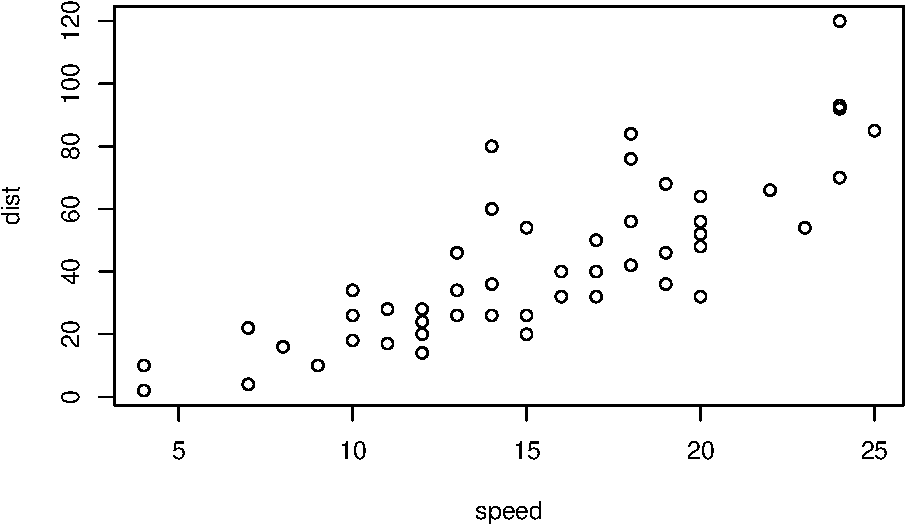
\includegraphics{_main_files/figure-latex/fig-margin-1.pdf}

\chapter{Introduction}\label{ch:intro}

You can label chapter and section titles using \texttt{\{\#label\}}
after them, e.g., we can reference Chapter \ref{ch:intro}. Let's use
chapter labels starting with ``ch:''.

Figures and tables with captions will be placed in \texttt{figure} and
\texttt{table} environments, respectively.

\begin{Shaded}
\begin{Highlighting}[]
\KeywordTok{par}\NormalTok{(}\DataTypeTok{mar =} \KeywordTok{c}\NormalTok{(}\DecValTok{4}\NormalTok{, }\DecValTok{4}\NormalTok{, }\FloatTok{.1}\NormalTok{, }\FloatTok{.1}\NormalTok{))}
\KeywordTok{plot}\NormalTok{(pressure, }\DataTypeTok{type =} \StringTok{'b'}\NormalTok{, }\DataTypeTok{pch =} \DecValTok{19}\NormalTok{)}
\end{Highlighting}
\end{Shaded}

\begin{figure}

{\centering 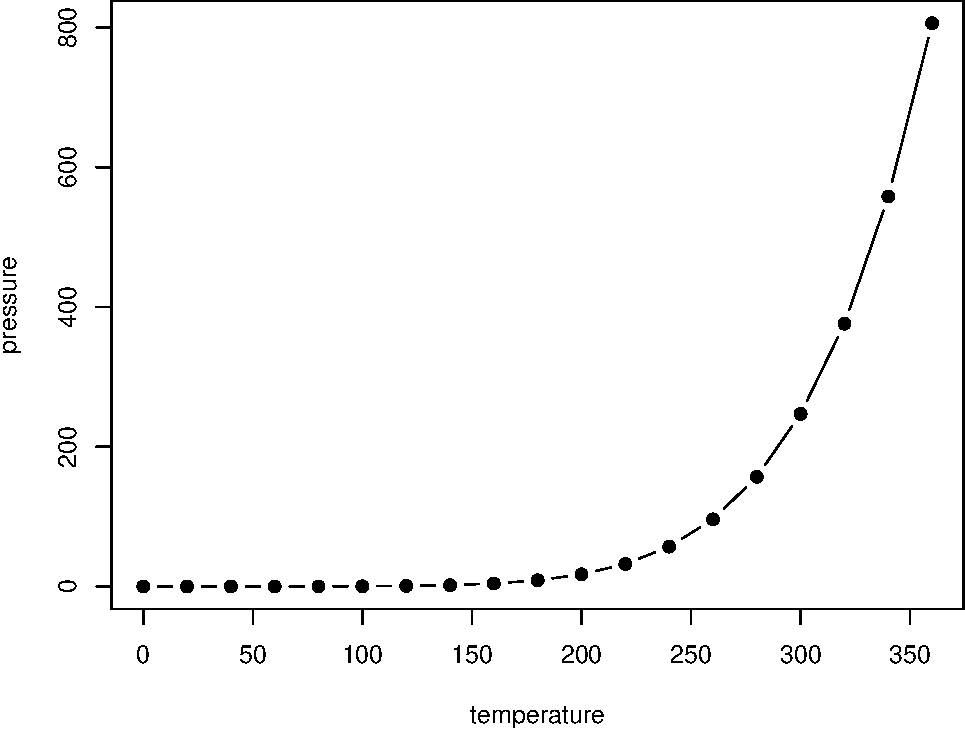
\includegraphics[width=0.8\linewidth]{_main_files/figure-latex/nice-fig-1} 

}

\caption{Here is a nice figure!}\label{fig:nice-fig}
\end{figure}

Reference a figure by its code chunk label with the \texttt{fig:}
prefix, e.g., see Figure \ref{fig:nice-fig}. Similarly, you can
reference tables generated from \texttt{knitr::kable()}, e.g., see Table
\ref{tab:nice-tab}.

\begin{Shaded}
\begin{Highlighting}[]
\NormalTok{knitr}\OperatorTok{::}\KeywordTok{kable}\NormalTok{(}
  \KeywordTok{head}\NormalTok{(iris, }\DecValTok{20}\NormalTok{), }\DataTypeTok{caption =} \StringTok{'Here is a nice table!'}\NormalTok{,}
  \DataTypeTok{booktabs =} \OtherTok{TRUE}
\NormalTok{)}
\end{Highlighting}
\end{Shaded}

\begin{table}

\caption{\label{tab:nice-tab}Here is a nice table!}
\centering
\begin{tabular}[t]{rrrrl}
\toprule
Sepal.Length & Sepal.Width & Petal.Length & Petal.Width & Species\\
\midrule
5.1 & 3.5 & 1.4 & 0.2 & setosa\\
4.9 & 3.0 & 1.4 & 0.2 & setosa\\
4.7 & 3.2 & 1.3 & 0.2 & setosa\\
4.6 & 3.1 & 1.5 & 0.2 & setosa\\
5.0 & 3.6 & 1.4 & 0.2 & setosa\\
\addlinespace
5.4 & 3.9 & 1.7 & 0.4 & setosa\\
4.6 & 3.4 & 1.4 & 0.3 & setosa\\
5.0 & 3.4 & 1.5 & 0.2 & setosa\\
4.4 & 2.9 & 1.4 & 0.2 & setosa\\
4.9 & 3.1 & 1.5 & 0.1 & setosa\\
\addlinespace
5.4 & 3.7 & 1.5 & 0.2 & setosa\\
4.8 & 3.4 & 1.6 & 0.2 & setosa\\
4.8 & 3.0 & 1.4 & 0.1 & setosa\\
4.3 & 3.0 & 1.1 & 0.1 & setosa\\
5.8 & 4.0 & 1.2 & 0.2 & setosa\\
\addlinespace
5.7 & 4.4 & 1.5 & 0.4 & setosa\\
5.4 & 3.9 & 1.3 & 0.4 & setosa\\
5.1 & 3.5 & 1.4 & 0.3 & setosa\\
5.7 & 3.8 & 1.7 & 0.3 & setosa\\
5.1 & 3.8 & 1.5 & 0.3 & setosa\\
\bottomrule
\end{tabular}
\end{table}

\hypertarget{refs}{}
\hypertarget{ref-dahlmanNakedStat2020}{}
Dahlman, C. (2020). Naked statistical evidence and incentives for lawful
conduct. \emph{International Journal of Evidence and Proof},
\emph{24}(2), 162--179.

\hypertarget{ref-diamond90}{}
Diamond, H. A. (1990). Reasonable doubt: To define, or not to define.
\emph{Columbia Law Review}, \emph{90}(6), 1716--1736.

\end{document}
